\chapter{Hardware} \label{sec:hardware}

This chapter will describe the hardware design of the device.

Starting point is the \emph{AD5933} by Analog Devices, an impedance converter IC that includes a digital-to-analog and
analog-to-digital converter, DSP engine for discrete time Fourier transform and internal clock source. It can output
frequencies in the range of \unit{10}{\hertz} to \unit{100}{\kilo\hertz} with the use of external clock sources.
A block diagram can be seen in \autoref{fig:ad_block}.

\begin{figure}[hpb]
  \centering
    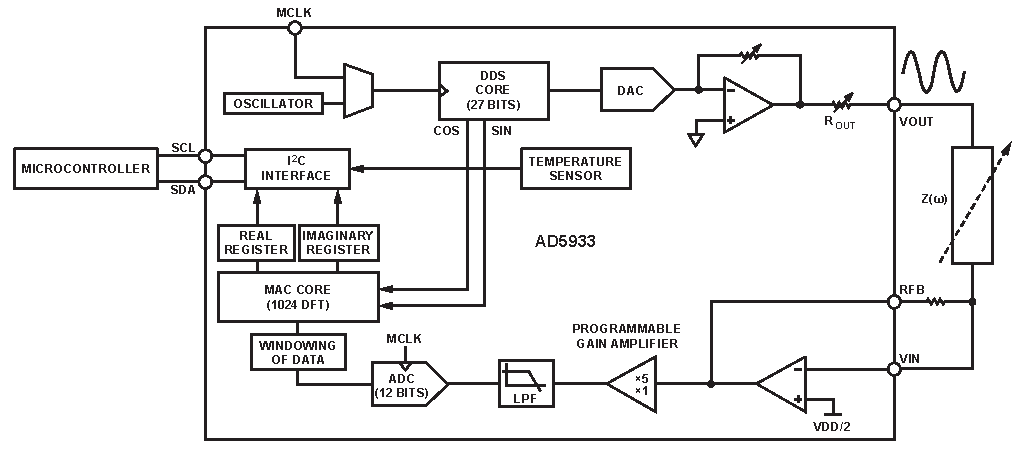
\includegraphics[width=\textwidth]{bilder/ad_block.pdf}
  \caption{Block diagram of the AD5933 showing the digital and analog parts connected to a micrcontroller
    and an impedance that is measured, respectively.}
  \label{fig:ad_block}
\end{figure}

For controlling the chip and interfacing with the PC, the \emph{STM32F4 Discovery} board by ST (see \autoref{fig:stm32})
is used. This is built around an STM32F407 microcontroller, includes two USB ports (one for programming and one for use
by the microcontroller), a programmer with debugging features and a clock source and exposes most of the microcontroller
pins on two $ 2 \times 25 $ pin headers. There are also some other peripherals which are not used for this project.

\begin{figure}[htpb]
  \centering
    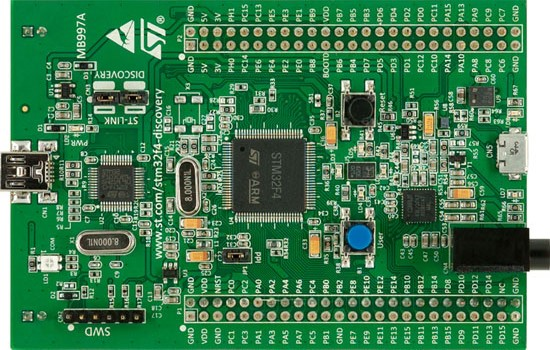
\includegraphics[width=0.6\textwidth]{bilder/stm32.jpg}
  \caption{STM32F4 Discovery board, USB port for debugging and programming on the left, USB port connected to the
    STM32F407 on the right.}
  \label{fig:stm32}
\end{figure}

The whole device consists of a single PCB onto which the STM32F4 Discovery board is mounted. This board has connections
for the measured impedances, a power supply jack as well as a header where calibration resistors are mounted.


\section{Analog Front End (AFE)}

The AD5933 has some severe limitations concerning its output and the load that can be placed there. Without additional
circuitry, the range is limited to at least a few \unit{100}{\kilo\ohm} up to \unit{10}{\mega\ohm}.
Since the desired range is down to about \unit{10}{\ohm}, and more than one impedance should be measured at once,
an external analog front end needs to be used.

A block diagram of the external AFE can be seen in \autoref{fig:schem_afe}. There are four analog multiplexers
(dual ADG725 by Analog Devices, M1 in the schematic) that connect multiple unknown and calibration impedances in a
four-wire arrangement, to cancel out the on-resistance of the multiplexers. Multiplexer M2 is used to attenuate the
output voltage of the AD5933, this is needed to measure small impedances so the output current is kept small.

\begin{figure}[hpb]
  \centering
    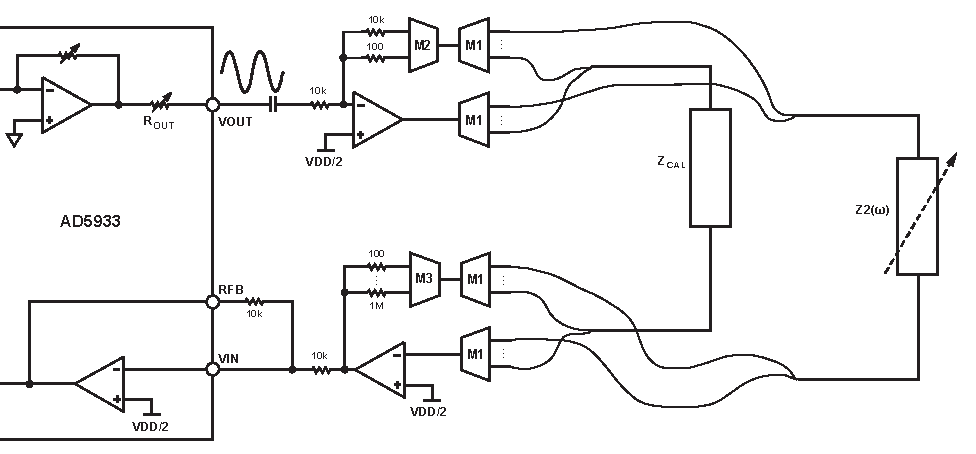
\includegraphics[width=\textwidth]{bilder/schem_afe.pdf}
  \caption{Block diagram of the AD5933 output stage with external analog front end.}
  \label{fig:schem_afe}
\end{figure}